\section*{Introduction}
La transcription automatique de la musique (TAM) est un défi ancien
\cite{first_one} et difficile qui n’est toujours pas résolu de manière
satisfaisante par les systèmes actuels. Il a engendré une
grande variété de sous-tâches qui ont donné naissance au domaine de la
recherche d’information musicale (RIM)\footnote{\url{https://ismir.net/}}.
Actuellement, en raison de la nature séquentielle et symbolique des données
musicales et du fait que les travaux en TAL sont assez avancés en analyse de
données séquentielles ainsi qu’en traitement du signal, de nombreux travaux de
RIM font appel au TAL. Certains de ces travaux se concentrent notamment sur
l’analyse des paroles de chansons\footnote{NLP4MuSA, the 2nd Workshop on
Natural Language Processing for Music and Spoken Audio, co-located with ISMIR
2021.}. <moi>Mais d’autres traitent directement la musique + ref.</moi>

Dans ce chapitre, nous parlerons de l’informatique musicale, nous montrerons
les liens existants entre le RIM et le TAL ainsi qu’entre les notions de
langage musical et langue naturelle. Nous traiterons également du problème de
l’AMT et de ses applications.

Enfin, nous décrirons les représentations de la musique qui sont nécessaires à
la compréhension du présent travail.
\section{Langues naturelles et musique en informatique}
COMPUTER MUSIC\\
L’informatique musicale ou \textit{Computer Music} regroupe l’ensemble des
méthodes permettant de créer ou d’analyser des données musicales à l’aide
d’outils informatiques \cite{book_muller}. Ce domaine implique l’utilisation de
méthodes numériques pour l’analyse et la synthèse de musique\footnote{Voir la
transformée de Fourier pour la musique dans \cite{fourier}}, qu’il s’agisse
d’informations audio, ou symboliques (aide à l’écriture, transcription, base de
partitions...). Un exemple de tâche dans ce domaine pourrait être l’analyse de
la structure de la musique et de la reconnaissance des accords\footnote{En
musique, un accord est un ensemble de notes considéré comme formant un tout du
point de vue de l’harmonie. Le plus souvent, ces notes sont jouées
simultanément ; mais les accords peuvent aussi s’exprimer par des notes
successive}.\\

RIM\\
La RIM est née du domaine de l’informatique musicale et apparaît vers le début
des années 2000 \cite{MIR_1}. L’objectif de cette science est la recherche et
l’extraction d’informations à partir de données musicales. Il s’agit d’un vaste
champ de recherche pluridisciplinaire, à l’intersection de acoustique, signal,
synthèse sonore, informatique, sciences cognitives, neurosciences, musicologie,
psycho-acoustique, etc. Cette discipline récente a notamment été soutenue par
de grandes entreprises technologiques\footnote{\url{
https://research.deezer.com/}} \footnote{\url{https://magenta.tensorflow.org/}}
\footnote{\url{https://research.atspotify.com/}} qui veulent développer des
systèmes de recommandation de musique ou des moteurs de recherche dédiés au son
et à la musique.\\

RIM et TAL \\
Aborder la musique comme un langage avec des méthodes de TAL nécessite une
réflexion autour de la musique en tant que langage ainsi que la possibilité de
comparer ce même langage avec les langues naturelles. Léonard Bernstein
\cite{lbernstein} a donné une série de six conférences publiques à Harvard
fondées en grande partie sur les théories linguistiques que Noam Chomsky a
exposées dans son livre « Language and Mind ». Lors de la première conférence,
qui a eu lieu le 9 octobre 1973, Bernstein a avoué être hanté par la notion
d’une grammaire musicale mondiale innée et il analyse dans ses trois premières
conférences, la musique en termes linguistiques (phonologie, syntaxe et
sémantique). Quelques travaux en neurosciences ont
également abordé ces questions, notamment par observation des processus
cognitifs et neuronaux que les systèmes de traitement de ces deux productions
humaines avaient en commun. Dans le travail de Poulin-Charronnat
\textit{et al.} \cite{poulincharronnat:hal-01985213}, la musique est reconnue
comme étant un système complexe spécifique à l’être humain dont une des
similitudes avec les langues naturelles est l’émergence de régularités
reconnues implicitement par le système cognitif. La question de la pertinence
de l’analogie entre langues naturelles et langage musical a également été
soulevée à l’occasion de projets de recherche en TAL. Keller \textit{et al.}
\cite{keller:hal-03279850} ont exploré le potentiel de ces techniques à travers
les plongements de mots et le mécanisme d’attention pour la modélisation de
données musicales. La question de la sémantique d’une phrase musicale apparaît,
selon eux, à la fois comme une limite et un défi majeur pour l’étude de cette
analogie. Ces considérations nous rapproche de la sémiologie de F. de Saussure
en tant que science générale des signes et dont la langue ne serait qu’un cas
particulier, caractérisé par l’arbitrariété totale de ses unités
\cite{wunderli2017ferdinand}.

\florent{exemples / illustration de la proximité thématique ?}

D’autres travaux
très récents, ont aussi été révélés lors de la \textit{première conférence sur
le NLP pour la musique et l’audio (NLP4MusA 2020)}. Lors de cette conférence,
Jiang \textit{et al.} \cite{Jiang2020DiscoveringMR} ont présenté leur
implémentation d’un modèle de langage musical visant à améliorer le mécanisme
d’attention par élément, déjà très largement utilisé dans les modèles de
séquence modernes pour le texte et la musique.\\
Le domaine du TAL qui se rapproche le plus du RIM est la reconnaissance de la
parole (Speech to text). En effet, la séparation des sources ont des approches
similaires dans les deux domaines. De plus, il existe un lien entre partition
musicale comme manière d’écrire la musique et texte comme manière d’écrire la
parole. La transcription musicale étant la notation d’une œuvre musicale
initialement non écrite, l’analogie avec l’écriture de la parole est aisée. Le
tableau \ref{spToTxt_vs_TAM} montre des différences et des similitudes entre
les deux domaines.

\begin{table}[h]
	\centering
	\begin{tabular}{|c|c|c|} \hline
	Domaines & Similitudes & Différences \\ \hline
	Speech to text & signal $\Rightarrow$ phonèmes $\Rightarrow$
    texte & données linéaires\\
	AMT & signal $\Rightarrow$ notes, accords $\Rightarrow$ partition & données
    structurées\\ \hline
	\end{tabular}
	\caption{speechToText vs AMT}
	\label{spToTxt_vs_TAM}
\end{table}
Non seulement les objectifs sont similaires, mais les problèmes et les
applications, eux aussi, sont comparables (transcription, synthèse, séparation
de sources, … ). Il faut néanmoins relever que les informations sont traitées
sont de nature différente (voir \textit{mettre ref vers sous-tâches comme beat
tracking et inférence de tempo en musique}).

\section{La transcription automatique de la musique}
1. OBJECTIF\\
Lorsqu’un musicien est chargé de créer une partition à partir d’un
enregistrement et qu’il écrit les notes qui composent le morceau en notation
musicale, on dit qu’il a créé une transcription musicale de cet enregistrement.
L’objectif de la TAM \cite{future_directions} est de convertir la performance
d’un musicien en notation musicale — à l’instar de la conversion de la parole
en texte dans le traitement du langage naturel. Cette définition peut être
comprise de deux manières différentes selon les articles scientifiques :
1) Processus de conversion d’un enregistrement audio en une notation pianoroll
(une représentation bidimensionnelle des notes de musique dans le temps)
2) Processus de conversion d’un enregistrement en notation musicale commune
\footnote{Ici, on parle de notation occidentale.} (c’est-à-dire une
partition).\\

2. APPLICATIONS\\
La TAM a des applications multiples \cite{future_directions} dont la plus
directe est de donner la possibilité à un musicien de générer la partition
d’une improvisation en temps réel afin de pouvoir reproduire sa performance
ultérieurement. Une autre application notable est la préservation du patrimoine
par exemple dans les styles musicaux où il n’existe peu de partitions (le
jazz, la pop, les musiques de tradition orale \footnote{ethno-musicologie}, …).
La TAM est aussi utile pour la recherche et l’annotation automatique
d’informations musicales, pour l’analyse musicologique\footnote{par exemple
par la constitution de corpus musicologiques} ou encore pour les systèmes
musicaux interactifs.

Un grand nombre de fichiers audio et vidéos musicaux sont disponibles sur le
Web, et pour la plupart d’entre eux, il est difficile de trouver les partitions
musicales correspondantes, qui sont pourtant nécessaires pour pratiquer la
musique, faire des reprises ou effectuer une analyse musicale détaillée.


Mais l’intérêt de la TAM est aussi d’avoir des partitions au contenu
exploitable, avec des formats texte ou XML (entre autres…) dont les données
sont manipulables, contrairement à de simples images en pdf
\footnote{Voir \url{https://archive.fosdem.org/2017/schedule/event/openscore/}
    et 0\_slides-Martin.pdf.}.\\

3. PROBLÈMES ET MÉTHODES SCIENTIFIQUES\\
L’analyse de la structure hiérarchique des séquences d’accords par utilisation
de modèles grammaticaux s’est avérée très utiles dans les analyses récentes de
l’harmonie du jazz \cite{harasimjazz}. Comme déjà évoqué précédemment, il
s’agit d’un problème ancien et difficile. C’est un « graal » de l’informatique
musicale. En 1976, H. C. Longuet-Higgins \cite{first_one} évoquait déjà la
représentation musicale en arbre syntaxique dans le but d’écrire
automatiquement des partitions à partir de données audio en se basant sur un
mimétisme psychologique de l’approche humaine.
La tâche de la TAM comprend deux activités distinctes : 1) l’analyse et la
représentation d’un morceau de musique ; 2) La génération d’une partition à
partir de la représentation du morceau.
 
\section{La transcription automatique de la batterie}
%\florent{tres bonne section}
La batterie est née au début du vingtième siècle \cite{histoire_drum_1}. C’est
donc un instrument récent qui s’est longtemps passé de partition. En effet
pour un batteur, la qualité de lecteur lorsqu’elle était nécessaire,
résidait essentiellement dans sa capacité à lire les partitions des autres
instrumentistes (par exemple, les grilles d’accords et la mélodie du thème en
jazz) afin d’improviser un accompagnement approprié que personne ne pouvait
écrire pour lui à sa place.
 
Les partitions de batterie sont arrivées par nécessité avec la pédagogie et
l’émergence d’écoles de batterie partout dans le monde. 
\florent{cite méthode et école Agostini ?}
Un autre facteur qui a contribué à l’expansion des partitions de batterie est
l’émergence de la musique assistée par ordinateur (MAO). En effet, l’usage de
boîtes à rythmes \footnote{Roland TR-808} ou de séquenceurs\footnote{SQ-1}
permettant d’expérimenter soi-même l’écriture de rythmes en les écoutant mixés
avec d’autres instruments sur des machines a permis aux compositeurs de
s’émanciper de la création d’un batteur en lui fournissant une partition
contenant les parties exactes qu’ils voulaient entendre sur leur musique.

La batterie a un statut à part dans l’univers de l’AMT puisqu’il s’agit
d’instruments sans hauteur (du point de vue harmonique), d’événements sonores
auxquels une durée est rarement attribuée et de notations spécifiques (symboles
des têtes de notes) \cite{Review_ADT}.

Les applications de la transcription automatique de la batterie (TAB) seraient
utiles, non seulement dans tous les domaines musicaux concernés par la batterie
dont certains manquent de partitions, notamment les musiques d’improvisation
\cite{future_directions}, mais aussi de manière plus générale dans le domaine
de la RIM : si les ordinateurs étaient capables d’analyser la partie de la
batterie dans la musique enregistrée, cela permettrait de faciliter de
nombreuses tâches de traitement de la musique liées au rythme. En particulier,
la détection et la classification des événements sonores de la batterie par des
méthodes informatiques est considérée comme un problème de recherche important
et stimulant dans le domaine plus large de la recherche d’informations
musicales \cite{Review_ADT}.\\
La TAB est un sujet de recherche crucial pour la compréhension des aspects
rythmiques de la musique, et a potentiellement un fort impact sur des domaines
plus larges tels que l’éducation musicale et la production musicale.

\section{Les représentations de la musique}
\florent{citer M. Müller FMP pour cette section?}

\subsection*{Les données audio}
\florent{trop technique. ne pas recopier wikipédia}
Le format de fichier WAV est une instance du \textit{Resource Interchange File
Format (RIFF)} défini par IBM et Microsoft. Le format RIFF agit comme une
"enveloppe" pour divers formats de codage audio. Un fichier WAV peux contenir
de l’audio compressé ou non compressé. 
\florent{LPCM pas utile ici. parle juste échantillons et compression.}
\florent{tu peux mentionner le format spectral (analyse harmonique) crucial en
MIR audio.}

\subsection*{Les données MIDI}
Le MIDI\footnote{\url{https://en.wikipedia.org/wiki/MIDI}} (Musical Instrument
Digital Interface) 
\florent{ne pas copier wikipédia verbatim. source: midi.org
         MIDI est un protocole temps réel pour échanger des messages (événement) et un format de fichier.}
est une norme technique qui décrit un protocole de communication, une interface numérique et des connecteurs électriques permettant de connecter une grande variété d’instruments de musique électroniques, d’ordinateurs et d’appareils audio connexes pour jouer, éditer et enregistrer de la musique.

\florent{fichier MIDI = séquence événements MIDI + dates (timestamp) ~ performance musicale symbolique}
\florent{donner ici les données des événements et expliquer ON/OFF (clavier)}
Les données midi sont représentées sous forme de piano-roll. 
%
Chaque point sur la figure \ref{piano_roll} est appelé « évènement MIDI » :
\begin{figure}[!h]
	\centering
	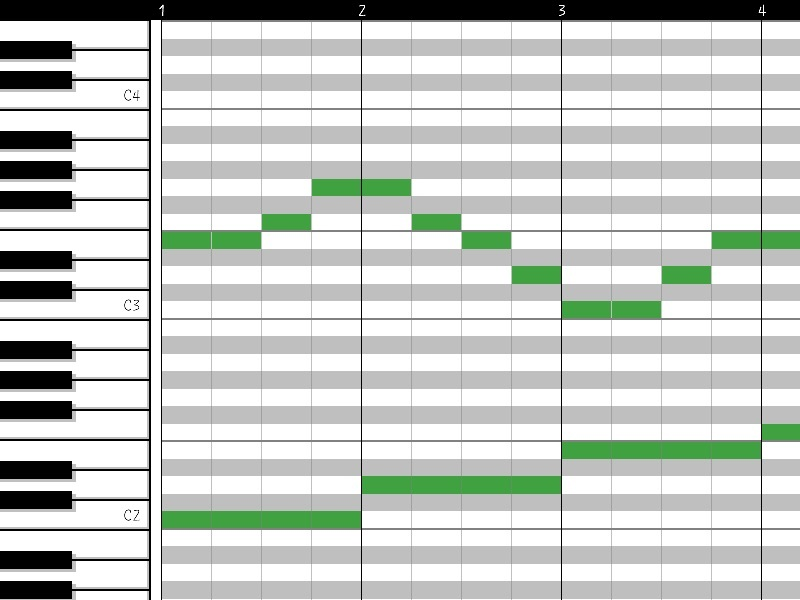
\includegraphics[height=40mm, width=50mm]{z_images/1_contexte/2_midi_piano.jpg}
	\caption{Exemple évènements avec durée}
	\label{piano_roll}
\end{figure}

Chaque évènement MIDI rassemble un ensemble d’informations sur la hauteur, la durée, le volume, etc… :
\begin{figure}[h!]
	\centering
	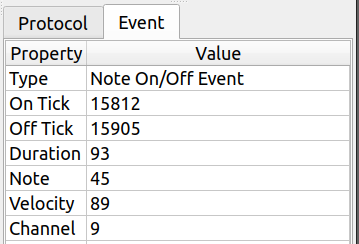
\includegraphics[height=40mm, width=50mm]{z_images/1_contexte/3_evenements_midi.png}
	\caption{Critère pour un évènement}
\end{figure} %\newpage
\florent{il n’y a pas de duration d’événement dans un MIDI file. 
         la "durée" est une distance entre 2 événemtns ON et OFF (c’est important dans ton travail).
         le screenshot n’est pas utile, écrit plutôt une liste itemize}

Pour la batterie, les évènements sont considérés sans durée, nous ignorerons donc les offsets (« Off Event »), les « Off Tick » et les « Duration ». 
Le \textit{channel} ne nous sera pas utile non plus.

\textit{Ici, définir Tick et channel.}

Voici un exemple de piano-roll midi pour la batterie :
\begin{figure}[h!]
	\centering
	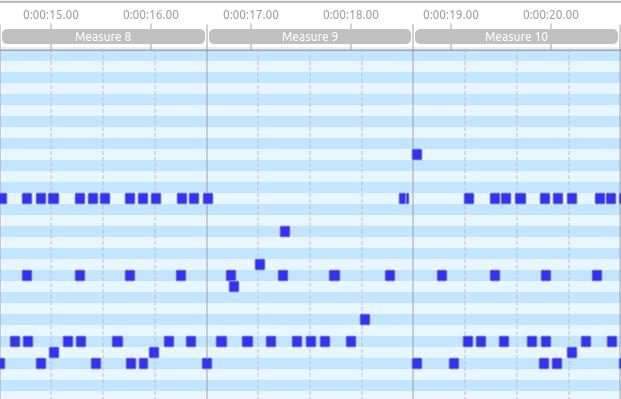
\includegraphics[height=40mm, width=50mm]{z_images/1_contexte/4_midi_batterie.png}
	\caption{Exemple évènements sans durée}
\end{figure}

On observe que toutes les durées sont identiques.
<dam>je te suggère un petit paragraphe ensuite, genre :
"Le format MIDI, originellement une norme technique, peut également être
considéré comme une représentation musicale. Celle-ci peut effectivement être
visualisée sous la forme d'une partition ou jouée par l'ordinateur. Ce format
historique, encore très largement utilisé, est très important (mais aussi
contraignant) dans le cadre de notre travail, dans la mesure où de nombreux
logiciels l'utilisent. Pour la transcription musicale, il constitue une strate
intermédiaire très utile entre le signal audio (enregistrement) et la
représentation musicale lisible par un humain (partition)"</dam>
\subsection*{Les partitions}
\florent{pour clarifier 3.1(sub les durées), décrire en 1.4 (ici) la notation
conventionnelles (piano etc) et 3.1(sub les durées) uniquement ce qui est
spécifique à la batterie, en expliquant les différences.}

\begin{figure}[h]
	\centering
	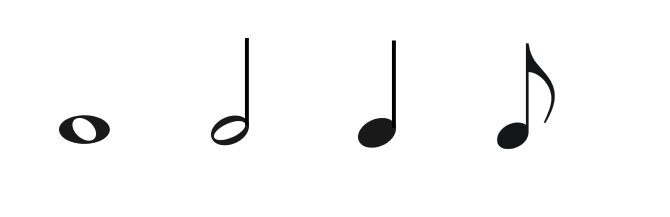
\includegraphics[height=10mm, width=25mm]{
    z_images/3_methodes/0_notation_de_la_batterie/0_figures_de_notes.png}
    \caption{}
    \label{4_notes}
\end{figure}
La figure \ref{4_notes} montre 4 figures de notes les plus courantes dont les
noms et les durées 
\florent{durées exprimées en unité de temps musicale, appelée le \emph{temps}, cf. section...}
sont respectivement, de gauche à droite :
\begin{itemize}
    \item La ronde, elle vaut 4 ; \florent{4 temps}
    \item La blanche, elle vaut 2 ;
    \item La noire, elle vaut 1 ;
    \item La croche, elle vaut 1/2.
\end{itemize}
Une figure de note \cite{danhauser} de musique combine plusieurs critères
\florent{plusieurs éléments}
\footnote{\url{https://fr.wikipedia.org/wiki/Note_de_musique}} :
\florent{plutôt que wikipedia cite Dannhauser ou autre ref. F.M. ou encore Gould 2011 Behind Bars}
\begin{itemize}
	\item Une tête de note :\\
	Sa position sur la portée indique la hauteur de la note. La tête de note
    peut aussi indiquer une durée.
	\item Une hampe :\\
	\florent{barre verticale liée à la tête de ntoe}
	Indicatrice d’appartenance à une voix en fonction de sa direction \florent{haut ou bas}
	et indicatrice d’une durée représentée par sa présence ou non (blanche ≠ ronde)
	\item Un crochet : La durée d’une note est divisée par deux à chaque
     crochet ajouté à la hampe d’une figure de note.
\end{itemize}
\begin{figure}[h]
	\centering
	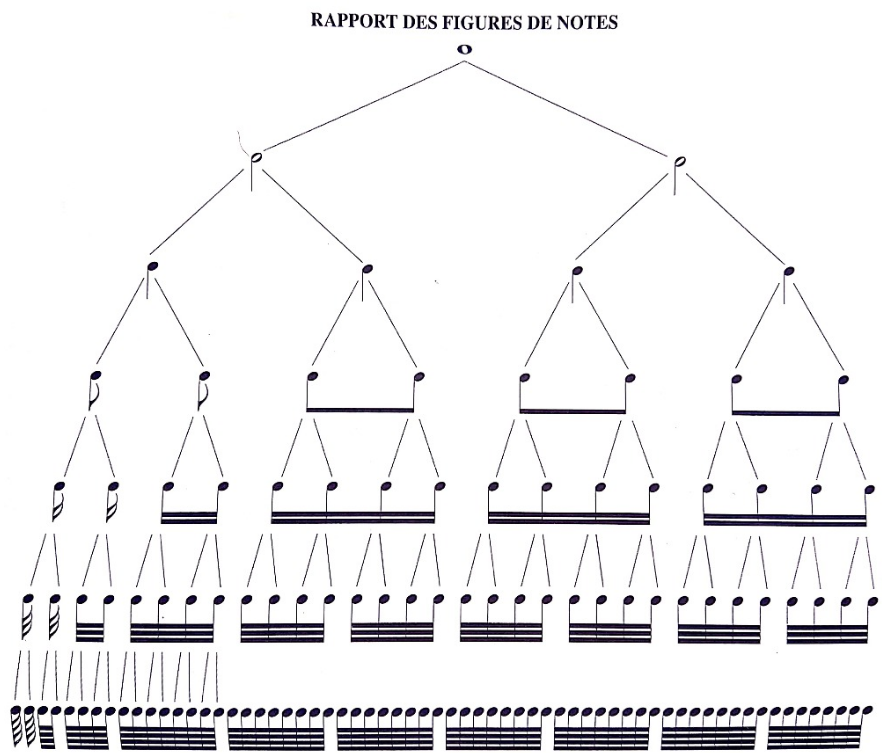
\includegraphics[height=50mm, width=80mm]{
    z_images/3_methodes/0_notation_de_la_batterie/1_rapport_figures_notes.png}
	\caption{Rapport des figures de notes}\cite{danhauser}
	\label{rapp_fig_notes}
\end{figure}

La figure \ref{rapp_fig_notes} montre les rapports de durée entre les figures de notes. Plus les durées sont longues, plus elles sont marquées par la tête de note (la note carrée fait deux fois la durée d’une ronde) ou la présence ou non de la hampe. À partir de la noire (3ème lignes en partant du haut), on ajoute un crochet à la hampe d’une figure de notes pour diviser sa durée par 2. 
Les notes à crochet (croche, double-croche, triple-croche…) 
peuvent être reliées ou non par des ligatures (voir les 4 dernières lignes de la figure \ref{rapp_fig_notes}).
\florent{ce premier paragraphe (jusqu'ici) est redondant avec \S 1.4 (sub. partitions). déplacer en 1.4?
         cf. proposition plus loin}


\begin{figure}[h!]
	\centering
	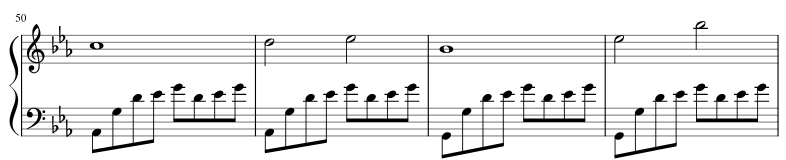
\includegraphics[height=30mm, width=120mm]{z_images/1_contexte/5_partition_piano.png}
	\caption{Exemple de partition de piano}
\end{figure}

Une partition de musique\footnote{\url{https://fr.wikipedia.org/wiki/Partition\_(musique)}} est un document qui porte la représentation systématique du langage musical sous forme écrite. Cette représentation est appelée transcription et elle sert à traduire les quatre caractéristiques du son musical :
\begin{itemize}
	\item la hauteur ;
	\item la durée ;
	\item l’intensité ;
	\item le timbre.
\end{itemize}
\florent{expliquer un peu plus avec exemple. 
ce serait mieux d’avoir un ex. avec des nuances, accents, appogiatures...}

Ainsi que de leurs combinaisons appelées à former l’ossature de l’œuvre musicale dans son déroulement temporel, à la fois :
\begin{itemize}
	\item diachronique (succession des instants, ce qui constitue en musique la mélodie) ;
	\item et synchronique (simultanéité des sons, c’est-à-dire l’harmonie).
\end{itemize}
\florent{explications sur l’aspect structuré (hiérarchie) : les mesures, les groupes ryhtmiques...
         c’est important ici}

\subsection*{Les formats XML}
Il existe plusieurs formats XML dédiés à la musique : MusicXML, MEI, MNX, …

L’inconvénient de ces formats est qu’ils sont verbeux et ambigus, c’est
pourquoi nous utilisons pour la transcription une représentation intermédiaire
abstraite décrite plus loin.


\begin{figure}[h]
	\centering
	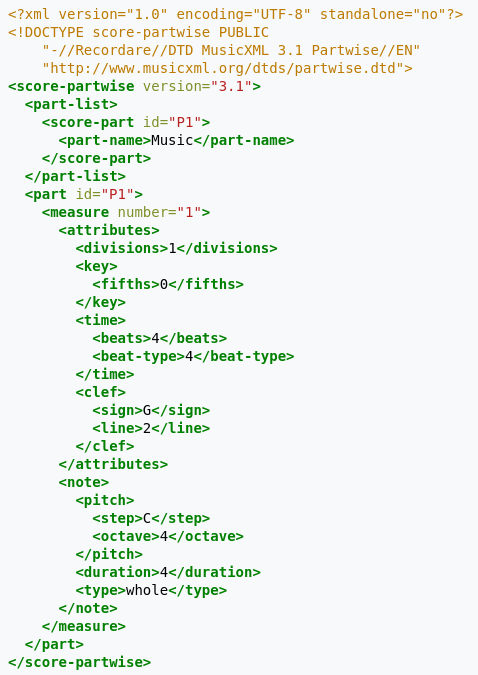
\includegraphics[height=50mm, width=50mm]{
    z_images/1_contexte/6_musicxml_0.png}
    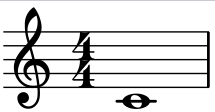
\includegraphics[height=20mm, width=40mm]{
    z_images/1_contexte/6_musicxml_1.png}
	\caption{MusicXML} 
	\label{MusicXML}
\end{figure}

Le figure \ref{MusicXML}
\footnote{\textit{Source images :
\url{https://fr.wikipedia.org/wiki/MusicXML}}}
représente un do en clef de sol de la durée d’une ronde sur une mesure en 4/4
écrit au format MusicXML.
Un des avantages de ce format est qu’il peut être converti aussi bien en
données MIDI qu’en partition musicale, ce qui en fait une interface
homme/machine.

\subsection*{appogiatures}
<flo>Parler des appogiatures ici ?</flo>
\subsection*{signature rythmique}
<flo>présenter rapidement la notation des signatures rythmiques</flo>

\section*{Conclusion}
Dans ce chapitre, nous avons établi que la RIM s’intéresse de plus en plus au
TAL, et que, par ce biais, il y a des liens possibles entre le langage musical
et les langues naturelles, le plus proche étant probablement le phénomène
d’écriture des sons de l’un comme de l’autre.

Nous avons également établi que la RIM est née de la TAM qui est un problème
ancien et très difficile et qu’il serait toujours très utile de le résoudre
(autant pour la TAM que pour la TAB).

Et enfin, nous avons décrit les représentations de la musique nécessaires à la
compréhension du présent mémoire, allant du son jusqu’à l’écriture.
